\begin{figure}[H]
    \centering


    \tikzset{every picture/.style={line width=0.75pt}} %set default line width to 0.75pt

    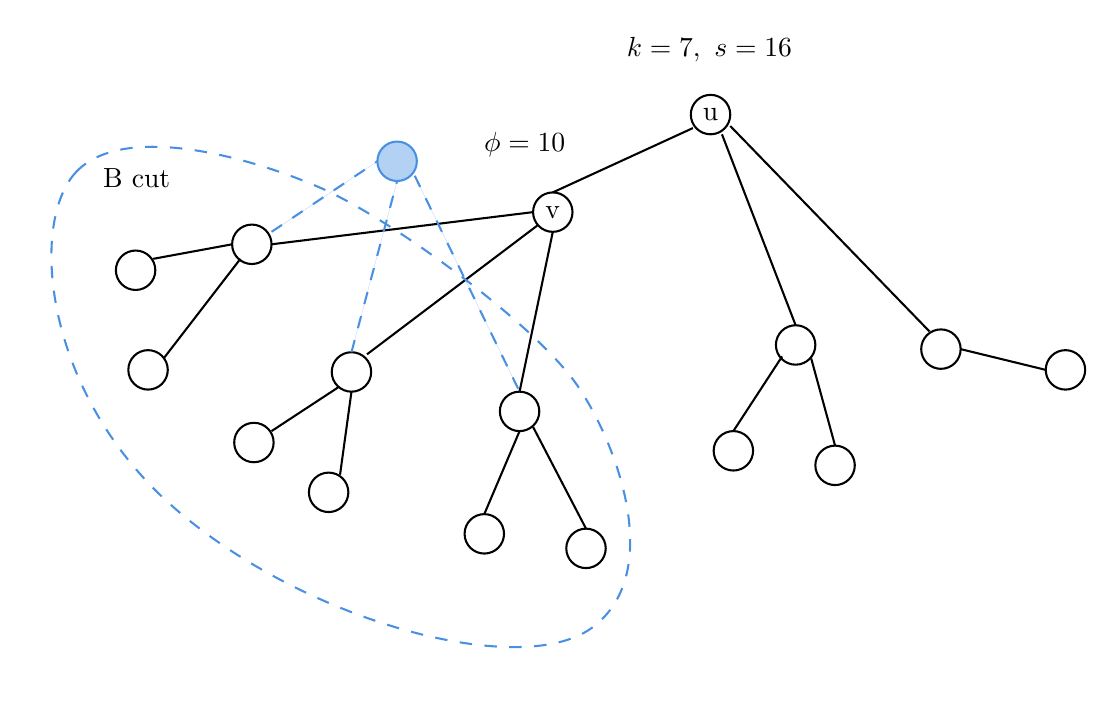
\begin{tikzpicture}[x=0.75pt,y=0.75pt,yscale=-1,xscale=1]
        %uncomment if require: \path (0,471); %set diagram left start at 0, and has height of 471

        %Shape: Circle [id:dp34076887970340053]
        \draw  [fill={rgb, 255:red, 255; green, 255; blue, 255 }  ,fill opacity=1 ] (392,61.5) .. controls (392,56.25) and (396.25,52) .. (401.5,52) .. controls (406.75,52) and (411,56.25) .. (411,61.5) .. controls (411,66.75) and (406.75,71) .. (401.5,71) .. controls (396.25,71) and (392,66.75) .. (392,61.5) -- cycle ;

        %Shape: Circle [id:dp9085081530378656]
        \draw  [fill={rgb, 255:red, 255; green, 255; blue, 255 }  ,fill opacity=1 ] (316,108.5) .. controls (316,103.25) and (320.25,99) .. (325.5,99) .. controls (330.75,99) and (335,103.25) .. (335,108.5) .. controls (335,113.75) and (330.75,118) .. (325.5,118) .. controls (320.25,118) and (316,113.75) .. (316,108.5) -- cycle ;

        %Shape: Circle [id:dp40613127689805917]
        \draw  [fill={rgb, 255:red, 255; green, 255; blue, 255 }  ,fill opacity=1 ] (403,223.5) .. controls (403,218.25) and (407.25,214) .. (412.5,214) .. controls (417.75,214) and (422,218.25) .. (422,223.5) .. controls (422,228.75) and (417.75,233) .. (412.5,233) .. controls (407.25,233) and (403,228.75) .. (403,223.5) -- cycle ;
        %Shape: Circle [id:dp9931876018636179]
        \draw  [fill={rgb, 255:red, 255; green, 255; blue, 255 }  ,fill opacity=1 ] (503,174.5) .. controls (503,169.25) and (507.25,165) .. (512.5,165) .. controls (517.75,165) and (522,169.25) .. (522,174.5) .. controls (522,179.75) and (517.75,184) .. (512.5,184) .. controls (507.25,184) and (503,179.75) .. (503,174.5) -- cycle ;
        %Shape: Circle [id:dp7698586857134941]
        \draw  [fill={rgb, 255:red, 255; green, 255; blue, 255 }  ,fill opacity=1 ] (563,184.5) .. controls (563,179.25) and (567.25,175) .. (572.5,175) .. controls (577.75,175) and (582,179.25) .. (582,184.5) .. controls (582,189.75) and (577.75,194) .. (572.5,194) .. controls (567.25,194) and (563,189.75) .. (563,184.5) -- cycle ;
        %Shape: Circle [id:dp07661905351809639]
        \draw  [fill={rgb, 255:red, 255; green, 255; blue, 255 }  ,fill opacity=1 ] (452,230.5) .. controls (452,225.25) and (456.25,221) .. (461.5,221) .. controls (466.75,221) and (471,225.25) .. (471,230.5) .. controls (471,235.75) and (466.75,240) .. (461.5,240) .. controls (456.25,240) and (452,235.75) .. (452,230.5) -- cycle ;
        %Shape: Circle [id:dp6823852359253104]
        \draw  [fill={rgb, 255:red, 255; green, 255; blue, 255 }  ,fill opacity=1 ] (433,172.5) .. controls (433,167.25) and (437.25,163) .. (442.5,163) .. controls (447.75,163) and (452,167.25) .. (452,172.5) .. controls (452,177.75) and (447.75,182) .. (442.5,182) .. controls (437.25,182) and (433,177.75) .. (433,172.5) -- cycle ;
        %Straight Lines [id:da2795330732074286]
        \draw    (407,71) -- (442.5,163) ;


        %Straight Lines [id:da95361289139327]
        \draw    (411,67) -- (507,166) ;


        %Straight Lines [id:da03919277897290474]
        \draw    (436,178) -- (412.5,214) ;


        %Straight Lines [id:da6790046753307697]
        \draw    (450,179) -- (461.5,221) ;


        %Straight Lines [id:da3674173158335614]
        \draw    (563,184.5) -- (522,174.5) ;


        %Straight Lines [id:da02933874590346841]
        \draw    (393,68) -- (325.5,99) ;


        %Shape: Circle [id:dp6930911043272474]
        \draw  [fill={rgb, 255:red, 255; green, 255; blue, 255 }  ,fill opacity=1 ] (172,219.5) .. controls (172,214.25) and (176.25,210) .. (181.5,210) .. controls (186.75,210) and (191,214.25) .. (191,219.5) .. controls (191,224.75) and (186.75,229) .. (181.5,229) .. controls (176.25,229) and (172,224.75) .. (172,219.5) -- cycle ;
        %Shape: Circle [id:dp4545176452788231]
        \draw  [fill={rgb, 255:red, 255; green, 255; blue, 255 }  ,fill opacity=1 ] (208,243.5) .. controls (208,238.25) and (212.25,234) .. (217.5,234) .. controls (222.75,234) and (227,238.25) .. (227,243.5) .. controls (227,248.75) and (222.75,253) .. (217.5,253) .. controls (212.25,253) and (208,248.75) .. (208,243.5) -- cycle ;
        %Shape: Circle [id:dp030374617759524325]
        \draw  [fill={rgb, 255:red, 255; green, 255; blue, 255 }  ,fill opacity=1 ] (219,185.5) .. controls (219,180.25) and (223.25,176) .. (228.5,176) .. controls (233.75,176) and (238,180.25) .. (238,185.5) .. controls (238,190.75) and (233.75,195) .. (228.5,195) .. controls (223.25,195) and (219,190.75) .. (219,185.5) -- cycle ;
        %Straight Lines [id:da016875084395338025]
        \draw    (222,193) -- (190,214) ;


        %Straight Lines [id:da7587321706433352]
        \draw    (228.5,195) -- (223,235) ;


        %Shape: Circle [id:dp6805190369347967]
        \draw  [fill={rgb, 255:red, 255; green, 255; blue, 255 }  ,fill opacity=1 ] (283,263.5) .. controls (283,258.25) and (287.25,254) .. (292.5,254) .. controls (297.75,254) and (302,258.25) .. (302,263.5) .. controls (302,268.75) and (297.75,273) .. (292.5,273) .. controls (287.25,273) and (283,268.75) .. (283,263.5) -- cycle ;
        %Shape: Circle [id:dp49294006336897334]
        \draw  [fill={rgb, 255:red, 255; green, 255; blue, 255 }  ,fill opacity=1 ] (332,270.5) .. controls (332,265.25) and (336.25,261) .. (341.5,261) .. controls (346.75,261) and (351,265.25) .. (351,270.5) .. controls (351,275.75) and (346.75,280) .. (341.5,280) .. controls (336.25,280) and (332,275.75) .. (332,270.5) -- cycle ;
        %Shape: Circle [id:dp4780933458297658]
        \draw  [fill={rgb, 255:red, 255; green, 255; blue, 255 }  ,fill opacity=1 ] (300,204.5) .. controls (300,199.25) and (304.25,195) .. (309.5,195) .. controls (314.75,195) and (319,199.25) .. (319,204.5) .. controls (319,209.75) and (314.75,214) .. (309.5,214) .. controls (304.25,214) and (300,209.75) .. (300,204.5) -- cycle ;
        %Straight Lines [id:da9579747847325664]
        \draw    (309.5,214) -- (292.5,254) ;


        %Straight Lines [id:da24682160488454663]
        \draw    (316,212) -- (341.5,261) ;


        %Straight Lines [id:da7254371683892009]
        \draw    (318,115) -- (236,177) ;


        %Straight Lines [id:da9361718285942648]
        \draw    (325.5,118) -- (309.5,195) ;


        %Shape: Circle [id:dp7136610740709559]
        \draw  [fill={rgb, 255:red, 255; green, 255; blue, 255 }  ,fill opacity=1 ] (171,124) .. controls (171,118.75) and (175.25,114.5) .. (180.5,114.5) .. controls (185.75,114.5) and (190,118.75) .. (190,124) .. controls (190,129.25) and (185.75,133.5) .. (180.5,133.5) .. controls (175.25,133.5) and (171,129.25) .. (171,124) -- cycle ;
        %Shape: Circle [id:dp7986023789770009]
        \draw  [fill={rgb, 255:red, 255; green, 255; blue, 255 }  ,fill opacity=1 ] (115,136.5) .. controls (115,131.25) and (119.25,127) .. (124.5,127) .. controls (129.75,127) and (134,131.25) .. (134,136.5) .. controls (134,141.75) and (129.75,146) .. (124.5,146) .. controls (119.25,146) and (115,141.75) .. (115,136.5) -- cycle ;
        %Straight Lines [id:da8486079993175883]
        \draw    (316,108.5) -- (190,124) ;


        %Straight Lines [id:da27547813733695325]
        \draw    (171,124) -- (133,131) ;


        %Shape: Circle [id:dp08981252883235546]
        \draw  [fill={rgb, 255:red, 255; green, 255; blue, 255 }  ,fill opacity=1 ] (121,184.5) .. controls (121,179.25) and (125.25,175) .. (130.5,175) .. controls (135.75,175) and (140,179.25) .. (140,184.5) .. controls (140,189.75) and (135.75,194) .. (130.5,194) .. controls (125.25,194) and (121,189.75) .. (121,184.5) -- cycle ;
        %Straight Lines [id:da22823959276419536]
        \draw    (175,131) -- (138,179) ;


        %Shape: Polygon Curved [id:ds15408437148876897]
        \draw  [color={rgb, 255:red, 74; green, 144; blue, 226 }  ,draw opacity=1 ][dash pattern={on 4.5pt off 4.5pt}] (96,89) .. controls (119,65) and (180,82) .. (214,97) .. controls (248,112) and (318,163) .. (338,193) .. controls (358,223) and (379,284) .. (344,309) .. controls (309,334) and (204,305) .. (142,250) .. controls (80,195) and (73,113) .. (96,89) -- cycle ;
        %Shape: Circle [id:dp5861650780323242]
        \draw  [color={rgb, 255:red, 74; green, 144; blue, 226 }  ,draw opacity=1 ][fill={rgb, 255:red, 179; green, 209; blue, 243 }  ,fill opacity=1 ] (241,84) .. controls (241,78.75) and (245.25,74.5) .. (250.5,74.5) .. controls (255.75,74.5) and (260,78.75) .. (260,84) .. controls (260,89.25) and (255.75,93.5) .. (250.5,93.5) .. controls (245.25,93.5) and (241,89.25) .. (241,84) -- cycle ;
        %Straight Lines [id:da880896354333569]
        \draw [color={rgb, 255:red, 74; green, 144; blue, 226 }  ,draw opacity=1 ][fill={rgb, 255:red, 74; green, 144; blue, 226 }  ,fill opacity=1 ] [dash pattern={on 4.5pt off 4.5pt}]  (190,118) -- (241,84) ;


        %Straight Lines [id:da2721999945811009]
        \draw [color={rgb, 255:red, 74; green, 144; blue, 226 }  ,draw opacity=1 ][fill={rgb, 255:red, 74; green, 144; blue, 226 }  ,fill opacity=1 ] [dash pattern={on 4.5pt off 4.5pt}]  (228.5,176) -- (250.5,93.5) ;


        %Straight Lines [id:da9627189828730469]
        \draw [color={rgb, 255:red, 74; green, 144; blue, 226 }  ,draw opacity=1 ][fill={rgb, 255:red, 74; green, 144; blue, 226 }  ,fill opacity=1 ] [dash pattern={on 4.5pt off 4.5pt}]  (259,91) -- (309.5,195) ;



        % Text Node
        \draw (401.5,61.5) node  [align=left] {u};
        % Text Node
        \draw (325.5,108.5) node  [align=left] {v};
        % Text Node
        \draw (312,76) node  [align=left] {$\displaystyle \phi =10$};
        % Text Node
        \draw (401,30) node [color={rgb, 255:red, 0; green, 0; blue, 0 }  ,opacity=1 ] [align=left] {$\displaystyle k=7,\ s=16$};
        % Text Node
        \draw (125,92) node  [align=left] {B cut};


    \end{tikzpicture}

    \caption{Example decompose step}\label{fig:decompose_example}
\end{figure}